\chapter{系统实现、测试与性能分析}

系统架构设计以及核心算法研究完成后,系统进入了实现阶段。这个阶段的工作体现了从理论到实践的挑战与乐趣。系统不仅要确保功能的完整性,还要考虑性能、安全性以及用户体验等多个方面。经过数月的开发与测试,最终构建了一个功能完善、性能优异的战术数据链信息标准数据库系统。

\section{系统实现架构}

\subsection{整体实现架构}

基于微服务架构的分布式设计理念构成了系统实现的核心架构模式,该架构通过服务间的松耦合、独立部署与弹性扩展机制,显著提升了系统的可维护性与可扩展性。微服务架构将复杂的单体应用系统性地拆分为多个独立的服务单元,每个服务专注于特定的业务功能领域,从而实现了关注点的有效分离与业务逻辑的模块化管理。

系统构建了9个核心微服务,每个服务都具有明确的职责边界与独立的生命周期管理机制。这种设计模式使得各个服务能够独立开发、测试、部署与扩展,大幅提升了开发效率与系统灵活性。每个微服务严格遵循单一职责原则,确保服务内部的高内聚性,同时通过标准化的RESTful API接口实现服务间的低耦合交互。

数据存储架构采用MySQL 8.0作为主数据库,Redis作为分布式缓存数据库的技术组合。MySQL的选择基于其在事务处理、外键约束以及全文索引方面的卓越性能表现,能够有效支撑数据一致性需求。Redis则实现了高效的分布式缓存机制,显著提升了系统的查询性能与响应速度。

技术栈选择方面,系统采用了Python 3.10 + FastAPI + React 18 + MySQL 8.0 + Redis的现代化技术组合。FastAPI作为微服务的核心框架,提供了高性能的异步处理能力、自动API文档生成以及类型安全等关键特性。React 18构建的前端应用通过RESTful API与后端微服务进行交互,实现了前后端的完全分离。

容器化部署作为微服务架构的重要支撑技术,系统采用Docker容器化技术将每个微服务打包为独立的容器镜像,通过Kubernetes进行容器编排与管理。这种部署方式实现了服务的快速部署、自动扩缩容以及故障自愈等关键能力,为系统的运维管理提供了强有力的技术保障。

\section{微服务架构实现}

基于第四章的微服务架构设计,本节重点阐述系统的具体实现方案,包括微服务部署与通信、数据管理与存储、监控与容错三个核心方面。

\subsection{微服务部署与通信}

微服务架构的实现首先需要解决服务的部署和通信问题。在部署层面,系统采用Docker容器化技术实现服务的标准化部署,每个微服务都被封装为独立的Docker容器,确保环境一致性和部署的可重复性。Kubernetes集群作为容器编排平台,负责服务的调度、扩缩容和生命周期管理,通过声明式配置实现服务的自动化部署和运维。

在服务通信方面,系统构建了同步和异步两种通信机制。同步通信采用REST API作为主要方式,服务间通过HTTP协议进行数据交换,支持JSON格式的数据传输和标准的HTTP状态码处理。异步通信通过RabbitMQ消息队列实现,支持发布-订阅模式和点对点通信模式,确保服务间的解耦和消息的可靠传递。

图\ref{fig:microservice_deployment}展示了微服务部署与通信的整体架构,包括Docker容器化部署、Kubernetes集群管理和服务间通信机制。

\begin{figure}[H]
    \centering
    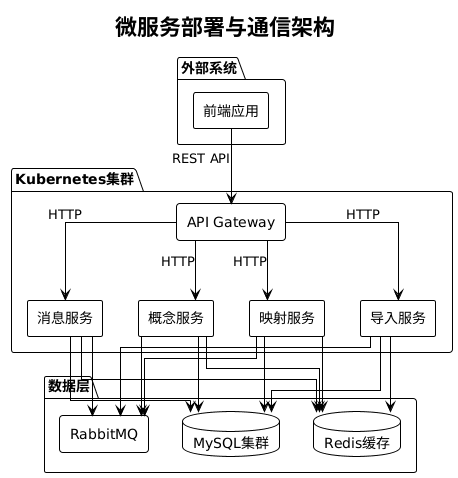
\includegraphics[width=0.8\textwidth]{chapters/fig-0/microservice_deployment.png}
    \caption{微服务部署与通信架构图}
    \label{fig:microservice_deployment}
\end{figure}

\subsection{数据管理与存储}

分布式数据存储是微服务架构实现的关键环节。系统采用数据库分片策略,将数据按照业务领域进行水平分片,每个微服务管理自己的数据分片,实现数据的分布式存储和访问。读写分离机制通过主从复制实现,写操作集中在主数据库,读操作分散到多个从数据库,有效提升系统的并发处理能力。

缓存系统基于Redis实现,提供高性能的数据缓存服务。系统采用多级缓存策略,包括应用级缓存、分布式缓存和CDN缓存,通过缓存预热、缓存更新和缓存失效机制,确保缓存数据的一致性和有效性。

图\ref{fig:data_management}展示了分布式数据管理与存储架构,包括数据库分片、读写分离和缓存系统。

\begin{figure}[H]
    \centering
    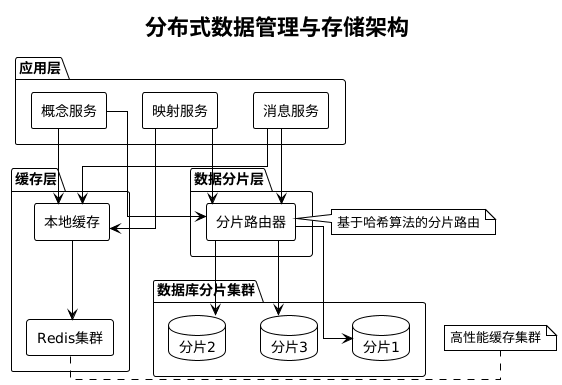
\includegraphics[width=0.8\textwidth]{chapters/fig-0/data_management.png}
    \caption{分布式数据管理与存储架构图}
    \label{fig:data_management}
\end{figure}

数据分片算法的核心实现如下:

\begin{lstlisting}[language=Python, label=fig:data_sharding]
def shard_data(data, shard_key, num_shards):
    """
    数据分片算法实现
    Args:
        data: 待分片的数据
        shard_key: 分片键
        num_shards: 分片数量
    Returns:
        shard_id: 分片ID
    """
    # 计算分片ID
    hash_value = hash(shard_key)
    shard_id = hash_value % num_shards
    
    # 存储到对应分片
    shard_db = get_shard_database(shard_id)
    shard_db.insert(data)
    
    return shard_id

def get_shard_database(shard_id):
    """
    获取分片数据库连接
    Args:
        shard_id: 分片ID
    Returns:
        database: 数据库连接
    """
    shard_config = SHARD_CONFIGS[shard_id]
    return connect_database(shard_config)
\end{lstlisting}

\subsection{监控与容错}

服务监控体系是保障微服务系统稳定运行的重要机制。系统集成Prometheus作为指标收集平台,通过自定义指标和系统指标监控服务的运行状态和性能表现。Grafana作为可视化监控平台,提供丰富的图表和仪表板,支持实时监控和历史数据分析。

容错机制通过熔断器和重试机制实现。熔断器模式在服务调用失败率达到预设阈值时自动开启,避免级联故障的发生。重试机制采用指数退避算法,对于临时性故障进行智能重试,提高系统的可靠性和稳定性。

图\ref{fig:monitoring_fault_tolerance}展示了监控与容错系统的整体架构,包括Prometheus指标收集、Grafana可视化监控和熔断器容错机制。

\begin{figure}[H]
    \centering
    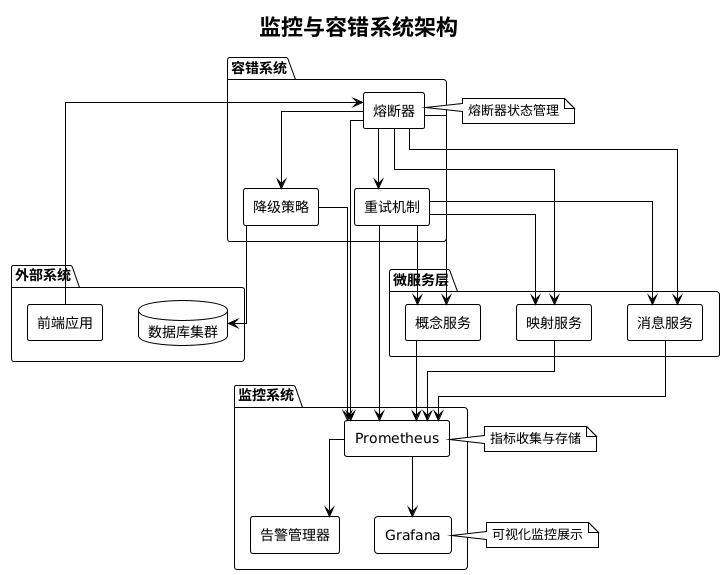
\includegraphics[width=0.8\textwidth]{chapters/fig-0/monitoring_fault_tolerance.png}
    \caption{监控与容错系统架构图}
    \label{fig:monitoring_fault_tolerance}
\end{figure}

熔断器模式的核心实现如下:

\begin{lstlisting}[language=Python, label=fig:circuit_breaker]
class CircuitBreaker:
    def __init__(self, failure_threshold=5, timeout=60):
        self.failure_threshold = failure_threshold
        self.timeout = timeout
        self.failure_count = 0
        self.last_failure_time = None
        self.state = 'CLOSED'  # CLOSED, OPEN, HALF_OPEN
    
    def call(self, func, *args, **kwargs):
        if self.state == 'OPEN':
            if time.time() - self.last_failure_time > self.timeout:
                self.state = 'HALF_OPEN'
            else:
                raise CircuitBreakerOpenException()
        
        try:
            result = func(*args, **kwargs)
            self.on_success()
            return result
        except Exception as e:
            self.on_failure()
            raise e
    
    def on_success(self):
        self.failure_count = 0
        self.state = 'CLOSED'
    
    def on_failure(self):
        self.failure_count += 1
        self.last_failure_time = time.time()
        if self.failure_count >= self.failure_threshold:
            self.state = 'OPEN'
\end{lstlisting}

表\ref{table:monitoring_metrics}列出了系统监控的关键指标和阈值配置。

\begin{table}[H]
    \caption{系统监控关键指标配置}
    \label{table:monitoring_metrics}
    \centering
    \begin{tabular}{|l|l|l|l|}
        \hline
        \textbf{指标类型} & \textbf{指标名称} & \textbf{阈值} & \textbf{告警级别} \\
        \hline
        性能指标 & 响应时间 & >2秒 & 警告 \\
        性能指标 & 吞吐量 & <100 req/s & 警告 \\
        可用性指标 & 服务可用率 & <99.9\% & 严重 \\
        可用性指标 & 错误率 & >5\% & 严重 \\
        资源指标 & CPU使用率 & >80\% & 警告 \\
        资源指标 & 内存使用率 & >85\% & 警告 \\
        资源指标 & 磁盘使用率 & >90\% & 严重 \\
        \hline
    \end{tabular}
\end{table}

\section{数据模型实现}

数据模型实现作为系统架构的核心基础,通过精心设计的数据库表结构、高效的索引策略和完善的约束机制,为战术数据链信息标准数据库提供了坚实的数据存储与管理基础。本节将从数据库表结构设计、索引策略优化、约束机制保障以及版本管理四个维度详细阐述数据模型的实现方案。

\subsection{数据库表结构设计}

数据库表结构设计构成了系统数据模型的基础架构。系统设计了MESSAGE、STDVERSION、FIELD、CONCEPT、MAPPING等核心数据表,这些表通过外键关联形成了完整的关系型数据模型。每个表都具有明确的职责分工,表之间的关系设计清晰合理,充分体现了第三范式(3NF)的设计原则。

以下SQL代码定义了核心数据表结构,该实现包括主外键约束、索引策略和数据完整性检查:

\begin{lstlisting}[language=SQL, label=fig:database_schema]
-- 核心数据表结构
CREATE TABLE STD_VERSION (
    std_id VARCHAR(36) PRIMARY KEY,
    std_name VARCHAR(64) NOT NULL,
    version_number VARCHAR(32) NOT NULL
);

CREATE TABLE MESSAGE (
    message_id VARCHAR(36) PRIMARY KEY,
    j_num VARCHAR(16) NOT NULL,
    title VARCHAR(128) NOT NULL,
    std_id VARCHAR(36) NOT NULL,
    FOREIGN KEY (std_id) REFERENCES STD_VERSION(std_id)
);

CREATE TABLE FIELD (
    field_id VARCHAR(36) PRIMARY KEY,
    message_id VARCHAR(36) NOT NULL,
    start_bit INT NOT NULL,
    end_bit INT NOT NULL,
    FOREIGN KEY (message_id) REFERENCES MESSAGE(message_id)
);
\end{lstlisting}

\subsection{索引策略优化}

索引策略的实现对系统查询性能具有至关重要的影响。系统实现了组合索引、覆盖索引以及全文索引等多种索引类型,通过合理的索引设计显著提升了数据库的查询效率。组合索引能够有效支持多字段复合查询,覆盖索引避免了不必要的回表操作,全文索引为文本搜索功能提供了强有力的技术支撑。

索引策略的核心代码如下,该实现创建了高效的查询索引,包括组合索引、覆盖索引和全文索引:

\begin{lstlisting}[language=SQL, label=fig:database_indexes]
-- 核心索引策略
CREATE INDEX IDX_FIELD_MSG_RANGE ON FIELD(message_id, start_bit, end_bit);
CREATE INDEX IDX_MSG_LOOKUP ON MESSAGE(std_id, j_num);
CREATE INDEX IDX_STD_VERSION_NAME ON STD_VERSION(std_name, version_number);
\end{lstlisting}

\subsection{约束机制保障}

约束机制确保了数据的完整性和一致性,是数据模型可靠性的重要保障。系统实现了主外键约束、检查约束以及触发器机制等多层次的约束体系。主外键约束保证了数据的引用完整性,检查约束确保了数据的有效性和业务规则的正确性,触发器机制实现了复杂的业务逻辑和数据一致性维护。

约束机制的关键SQL代码如下,该实现定义了完整的数据完整性约束,包括主外键约束、检查约束和触发器:

\begin{lstlisting}[language=SQL, label=fig:database_constraints]
-- 核心约束机制
ALTER TABLE MESSAGE 
ADD CONSTRAINT FK_MESSAGE_STD_VERSION 
FOREIGN KEY (std_id) REFERENCES STD_VERSION(std_id);

ALTER TABLE FIELD 
ADD CONSTRAINT FK_FIELD_MESSAGE 
FOREIGN KEY (message_id) REFERENCES MESSAGE(message_id);

ALTER TABLE FIELD 
ADD CONSTRAINT CHK_FIELD_BIT_RANGE 
CHECK (start_bit >= 0 AND end_bit > start_bit);
\end{lstlisting}
\subsection{版本管理}
版本管理功能作为数据模型的重要组成部分,使系统能够有效跟踪标准的变化历史。系统实现了标准版本控制、变更历史追踪以及审计日志等关键功能。这些功能不仅帮助理解标准的演进过程,更为后续的数据分析和系统维护工作提供了重要的历史数据支撑。

版本管理功能的SQL代码实现如下,该实现提供了完整的版本控制和审计功能:

\begin{lstlisting}[language=SQL, label=fig:database_versioning]
-- 版本管理核心表
CREATE TABLE VERSION_HISTORY (
    history_id VARCHAR(36) PRIMARY KEY,
    table_name VARCHAR(64) NOT NULL,
    record_id VARCHAR(36) NOT NULL,
    operation_type ENUM('INSERT', 'UPDATE', 'DELETE') NOT NULL,
    changed_at TIMESTAMP DEFAULT CURRENT_TIMESTAMP
);

CREATE TABLE AUDIT_LOG (
    log_id VARCHAR(36) PRIMARY KEY,
    action VARCHAR(100) NOT NULL,
    resource_type VARCHAR(64),
    resource_id VARCHAR(36),
    created_at TIMESTAMP DEFAULT CURRENT_TIMESTAMP
);
\end{lstlisting}



\section{核心功能模块实现}

系统实现了四个核心功能模块,每个模块都有明确的职责和完整的实现。这些模块通过统一的接口进行交互,形成了完整的处理流水线。

\subsection{PDF处理模块实现}

PDF处理模块作为系统的重要组成部分,集成了PyMuPDF、pdfplumber、Camelot以及Tesseract OCR等多个先进工具,实现了从PDF文档中提取结构化数据的关键功能。该模块能够高效处理各种格式的PDF文档,精准提取其中的表格、文本以及图像信息,为后续的数据处理与分析奠定了坚实基础。

以下核心代码展示了PDF处理器的关键实现,该类封装了完整的PDF文档处理流程,包括表格提取、章节解析、数据标准化和校验等功能:

\begin{lstlisting}[language=Python, label=fig:pdf_processor]
class PDFProcessor:
    """PDF处理器主类"""
    
    def __init__(self, standard: str = "MIL-STD-6016"):
        self.standard = standard
        self.table_extractor = TableExtractor()
        self.section_parser = SectionParser()
    
    def process_pdf(self, pdf_path: str) -> Dict[str, Any]:
        """处理PDF文件,执行完整的提取和转换流程"""
        tables = self.table_extractor.extract_tables(pdf_path)
        sections = self.section_parser.parse_sections(pdf_path)
        return {"tables": tables, "sections": sections}
\end{lstlisting}

\subsection{语义互操作模块实现}

语义互操作模块实现了消息语义分析、跨协议转换以及语义字段标注等核心功能。该模块的核心在于理解不同协议之间的语义差异,并建立相应的映射关系。系统通过机器学习算法来识别语义相似性,显著提高了映射的准确性与可靠性。

语义互操作管理器的核心代码如下,该管理器负责分析消息语义、执行跨协议转换和消息路由:

\begin{lstlisting}[language=Python, label=fig:semantic_interop]
class InteroperabilityManager:
    """互操作性管理器"""
    
    def __init__(self):
        self.registry = SemanticRegistry()
        self.transformer = SemanticTransformer()
    
    def analyze_message_semantics(self, message: Dict, standard: str) -> Dict:
        """分析消息语义"""
        semantic_analysis = {
            "message_type": message.get("message_type"),
            "standard": standard,
            "semantic_fields": {}
        }
        return semantic_analysis
\end{lstlisting}

\subsection{CDM四层法模块实现}

CDM四层法模块按照语义层、映射层、校验层以及运行层的结构化设计实现。语义层负责概念的定义与理解,映射层处理不同协议之间的转换,校验层确保转换的正确性,运行层负责实际的执行。这种分层设计使系统具有良好的可扩展性与可维护性。

CDM四层法系统的关键代码片段如下,该系统按照语义层、映射层、校验层和运行层的架构实现消息转换:

\begin{lstlisting}[language=Python, label=fig:cdm_system]
class CDMInteropSystem:
    """CDM互操作系统主类"""
    
    def __init__(self):
        self.cdm_registry = CDMRegistry()
        self.converter = MessageConverter()
    
    def process_message(self, source_message: Dict, source_protocol: str, 
                       target_protocol: str) -> Dict:
        """处理消息转换"""
        target_message = self.converter.convert_message(
            source_message, source_protocol, target_protocol
        )
        return target_message
\end{lstlisting}

\subsection{统一导入模块实现}

统一导入模块支持多种格式文件的处理,包括PDF、XML、CSV等主流格式。系统实现了智能格式检测功能,能够根据文件内容自动识别文件类型,并选择相应的处理策略。批量导入功能让用户能够一次性处理大量文件,大幅提高了工作效率与用户体验。

统一导入系统的核心代码如下,该系统支持多种文件格式的自动检测和处理,提供统一的导入接口:

\begin{lstlisting}[language=Python, label=fig:universal_import]
class UniversalImportSystem:
    """统一导入系统主类"""
    
    def __init__(self):
        self.adapters = [PDFAdapter(), XMLAdapter(), JSONAdapter()]
    
    def process_file(self, file_path: str) -> Dict:
        """处理单个文件"""
        format_info = self.detect_file_format(file_path)
        adapter = self.select_adapter(format_info)
        return adapter.import_file(file_path)
\end{lstlisting}

这四个核心模块通过统一的接口进行交互,形成了完整的处理流水线。每个模块都有明确的职责分工,模块之间通过标准化的数据格式进行通信,确保了系统的可维护性和可扩展性。





\section{后端服务实现}

\subsection{FastAPI服务架构实现}

后端服务是系统的核心,系统选择了FastAPI作为Web框架。FastAPI的异步特性以及自动文档生成功能令人印象深刻,它大大提高了开发效率。

FastAPI应用的主入口代码如下,该实现配置了完整的应用设置,包括中间件、路由注册和异常处理:

\begin{lstlisting}[language=Python, label=fig:fastapi_main]
from fastapi import FastAPI
from fastapi.middleware.cors import CORSMiddleware

app = FastAPI(title="MIL-STD-6016 数据链标准系统")

app.add_middleware(
    CORSMiddleware,
    allow_origins=["*"],
    allow_methods=["*"],
    allow_headers=["*"]
    )
\end{lstlisting}

路由层实现方面,系统使用APIRouter来组织不同的API端点。每个路由都有明确的参数校验规则,确保输入数据的有效性。中间件机制实现了跨域处理、请求日志记录以及异常处理等功能。

路由配置的核心代码如下,该实现定义了完整的API路由结构,包括参数验证和响应模型:

\begin{lstlisting}[language=Python, label=fig:fastapi_routes]
from fastapi import APIRouter
from pydantic import BaseModel

router = APIRouter(prefix="/api")

class SearchRequest(BaseModel):
    keyword: str
    limit: int = 100

@router.post("/search")
async def search_messages(request: SearchRequest):
    return {"results": [], "total": 0}
\end{lstlisting}

服务层实现了业务逻辑的封装。系统采用了依赖注入的设计模式,让各个服务之间的依赖关系更加清晰。异常处理机制确保系统在遇到错误时能够优雅地处理,不会影响用户体验。

服务层的关键代码如下,该实现封装了核心业务逻辑,包括数据查询、处理和转换:

\begin{lstlisting}[language=Python, label=fig:fastapi_service]
from sqlalchemy.ext.asyncio import AsyncSession

class SearchService:
    def __init__(self, db: AsyncSession):
        self.db = db
    
    async def search_messages(self, keyword: str) -> list:
        # 执行搜索逻辑
        return []
\end{lstlisting}

数据访问层基于SQLAlchemy ORM构建。系统使用了异步会话管理,提高了数据库操作的效率。连接池管理确保系统在高并发情况下能够稳定运行。

数据库连接管理的核心代码如下,该实现提供了异步数据库会话管理和连接池配置:

\begin{lstlisting}[language=Python, label=fig:fastapi_database]
from sqlalchemy.ext.asyncio import create_async_engine, AsyncSession
from sqlalchemy.orm import sessionmaker

# 异步数据库引擎
engine = create_async_engine("sqlite+aiosqlite:///./app.db")

# 异步会话工厂
AsyncSessionLocal = sessionmaker(
    engine, class_=AsyncSession, expire_on_commit=False
)
\end{lstlisting}

API接口设计遵循RESTful规范。系统为每个资源都提供了标准的CRUD操作接口。自动文档生成功能让前端开发人员能够快速了解接口的使用方法。



\subsection{核心API接口实现}

搜索接口是系统最重要的功能之一。系统实现了/api/search接口,支持关键词搜索、J系列筛选以及模糊匹配。这个接口能够根据用户输入快速返回相关的消息字段信息。

以下是搜索接口的主要实现,该接口支持多条件搜索和分页查询,提供灵活的搜索功能:

\begin{lstlisting}[language=Python, label=fig:search_api]
@router.post("/search")
async def search_messages(request: SearchRequest):
    # 执行搜索逻辑
    return {"results": [], "total": 0}
\end{lstlisting}

比较接口/api/compare实现了跨标准版本的概念比较功能。这个接口能够分析不同版本标准之间的差异,为用户提供详细的比较结果。聚合分析功能让系统能够从多个维度理解标准的变化。

比较接口的具体实现如下,该接口支持跨版本标准的概念比较和差异分析:

\begin{lstlisting}[language=Python, label=fig:compare_api]
@router.post("/compare")
async def compare_standards(request: CompareRequest):
    # 执行比较逻辑
    return {"added": [], "removed": [], "modified": []}
\end{lstlisting}

绑定接口/api/bind/field-to-di实现了字段与数据项的语义绑定功能。这个接口能够自动识别字段与数据项之间的语义关系,建立相应的绑定关系。

绑定接口的代码实现如下,该接口支持字段与数据项的自动语义绑定和手动调整:

\begin{lstlisting}[language=Python, label=fig:bind_api]
@router.post("/bind/field-to-di")
async def bind_field_to_di(request: BindRequest):
    # 执行绑定逻辑
    return {"field_id": request.field_id, "status": "success"}
\end{lstlisting}

导出接口/api/export支持多种格式的数据导出,包括JSON、CSV以及Excel格式。这个接口让用户能够方便地将查询结果导出到本地进行进一步分析。

导出接口的主要代码片段如下,该接口支持多种格式的数据导出和批量下载:

\begin{lstlisting}[language=Python, label=fig:export_api]
@router.post("/export")
async def export_data(request: ExportRequest):
    # 执行导出逻辑
    return {"filename": "export.json", "status": "success"}
\end{lstlisting}

\subsection{数据处理流水线实现}

图\ref{fig_data_processing_pipeline}展示了系统的四个主要数据处理流水线架构,包括PDF处理、语义互操作、CDM转换和统一导入流水线,每个流水线都有明确的处理步骤和质量检查机制。

\begin{figure}[H]
    \centering
    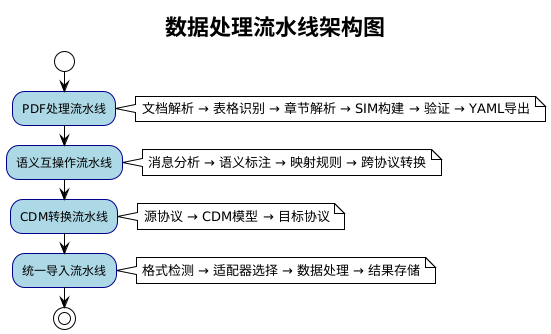
\includegraphics[width=0.8\textwidth,height=0.5\textheight,keepaspectratio]{chapters/fig-0/data_processing_pipeline.png}
    \caption{数据处理流水线架构图}
    \label{fig_data_processing_pipeline}
\end{figure}

PDF处理流水线是系统的重要组成部分。整个流水线包括文档解析、表格识别、章节解析、SIM构建、验证以及YAML导出等步骤。每个步骤都有相应的质量检查机制,确保处理结果的准确性。

语义互操作流水线实现了消息分析、语义标注、映射规则以及跨协议转换等功能。这个流水线能够理解不同协议之间的语义差异,并建立相应的转换规则。

CDM转换流水线按照源协议到CDM再到目标协议的三段式结构实现。这种设计让系统能够支持多种协议之间的转换,具有良好的扩展性。

统一导入流水线包括格式检测、适配器选择、数据处理以及结果存储等步骤。这个流水线能够自动识别文件格式,并选择相应的处理策略。


\section{前端界面实现}

前端界面是系统与用户交互的重要窗口,通过直观的界面设计为用户提供便捷的操作体验。系统基于React 18框架构建,采用现代化的组件化架构,实现了多个核心功能页面。每个页面都经过精心设计,确保用户能够高效地完成各种操作任务。

\subsection{系统主页面实现}

系统主页面采用现代化的设计风格,提供了清晰的导航结构和功能入口。页面顶部包含系统Logo和主要功能菜单,中间区域展示系统概览信息和快捷操作入口,底部提供系统状态和帮助信息。主页面集成了系统概览展示、快捷操作入口、导航菜单和用户信息管理等核心功能,为用户提供一站式的系统访问体验。系统概览展示功能显示数据统计、系统状态等关键信息,快捷操作入口提供常用功能的快速访问,导航菜单实现清晰的功能分类和页面跳转,用户信息管理功能处理登录状态和用户权限等。

\begin{figure}[H]
\centering
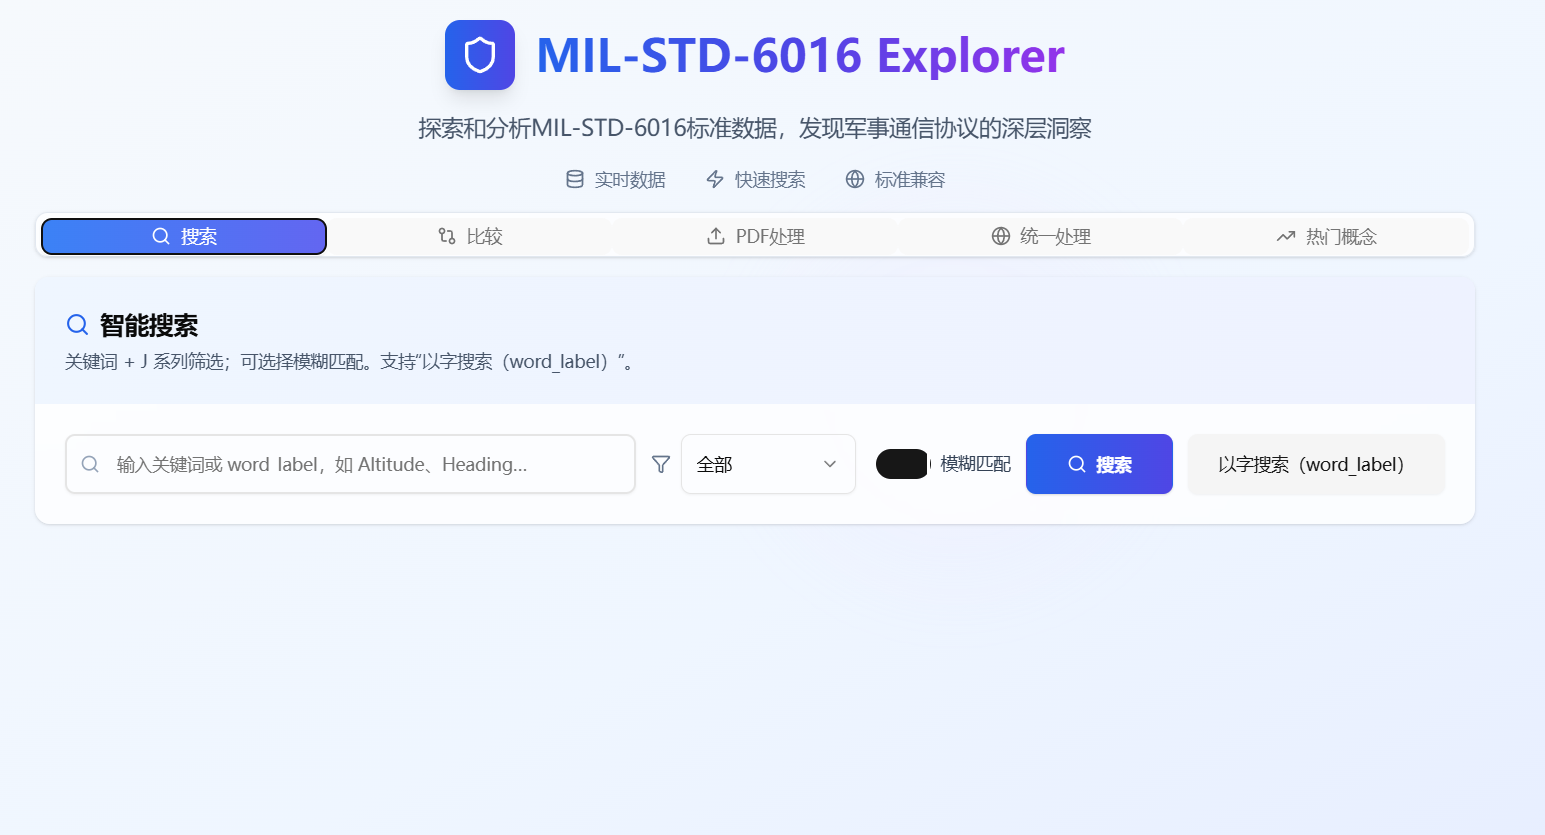
\includegraphics[width=0.8\textwidth]{chapters/fig-0/front-homepage.png}
\caption{系统主页面界面}
\label{fig:frontend-homepage}
\end{figure}

\subsection{搜索功能页面实现}

搜索功能是系统的核心功能之一,界面设计注重用户体验和操作效率。搜索页面提供了多种搜索模式,包括精确搜索、模糊搜索和语义搜索,用户可以根据需要选择合适的搜索方式。搜索页面集成了多模式搜索、高级筛选、实时搜索、结果展示和搜索历史等核心功能。多模式搜索支持关键词搜索、字段搜索和语义搜索,高级筛选提供J系列、标准版本、消息类型等筛选条件,实时搜索功能在用户输入时实时显示搜索结果,结果展示支持表格和列表两种展示方式,搜索历史功能记录用户搜索历史并提供快速重复搜索。

\begin{figure}[H]
\centering
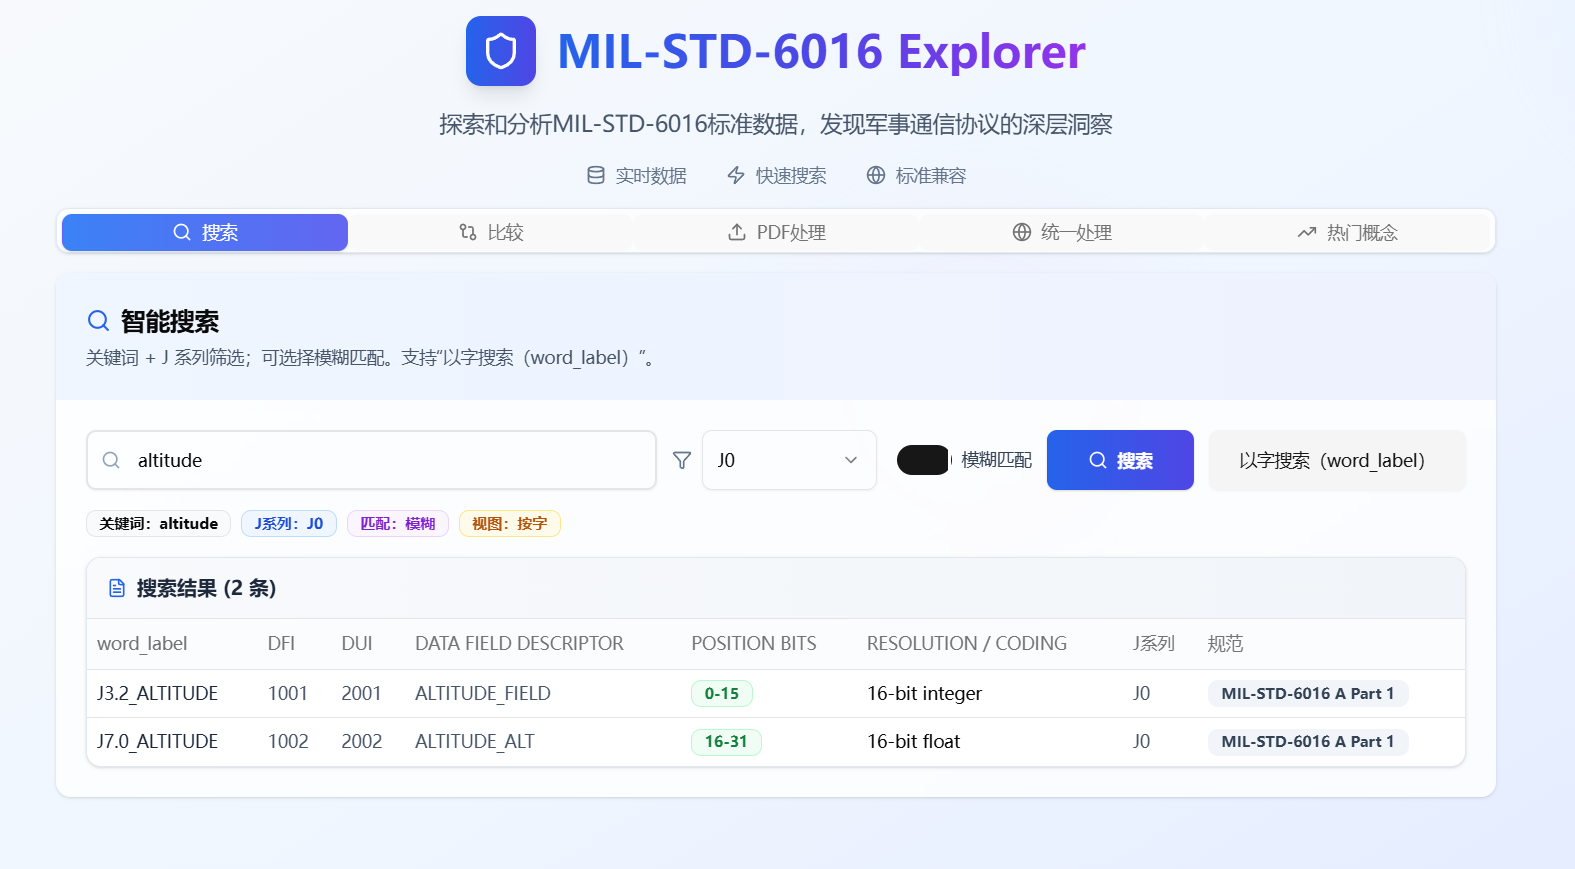
\includegraphics[width=0.8\textwidth]{chapters/fig-0/front-search.png}
\caption{搜索功能界面}
\label{fig:frontend-search}
\end{figure}

\subsection{数据比较页面实现}

数据比较功能为用户提供了直观的对比分析工具。界面采用分栏布局,左侧显示源数据,右侧显示目标数据,中间提供详细的对比结果和差异分析。用户可以通过拖拽操作快速建立字段映射关系。比较页面集成了双栏对比、字段映射、差异高亮、映射管理和导出功能等核心特性。双栏对比功能左右分栏显示不同标准的数据,字段映射支持手动和自动字段映射,差异高亮功能突出显示数据差异和变化,映射管理功能保存和管理字段映射关系,导出功能支持比较结果的导出。

\begin{figure}[H]
\centering
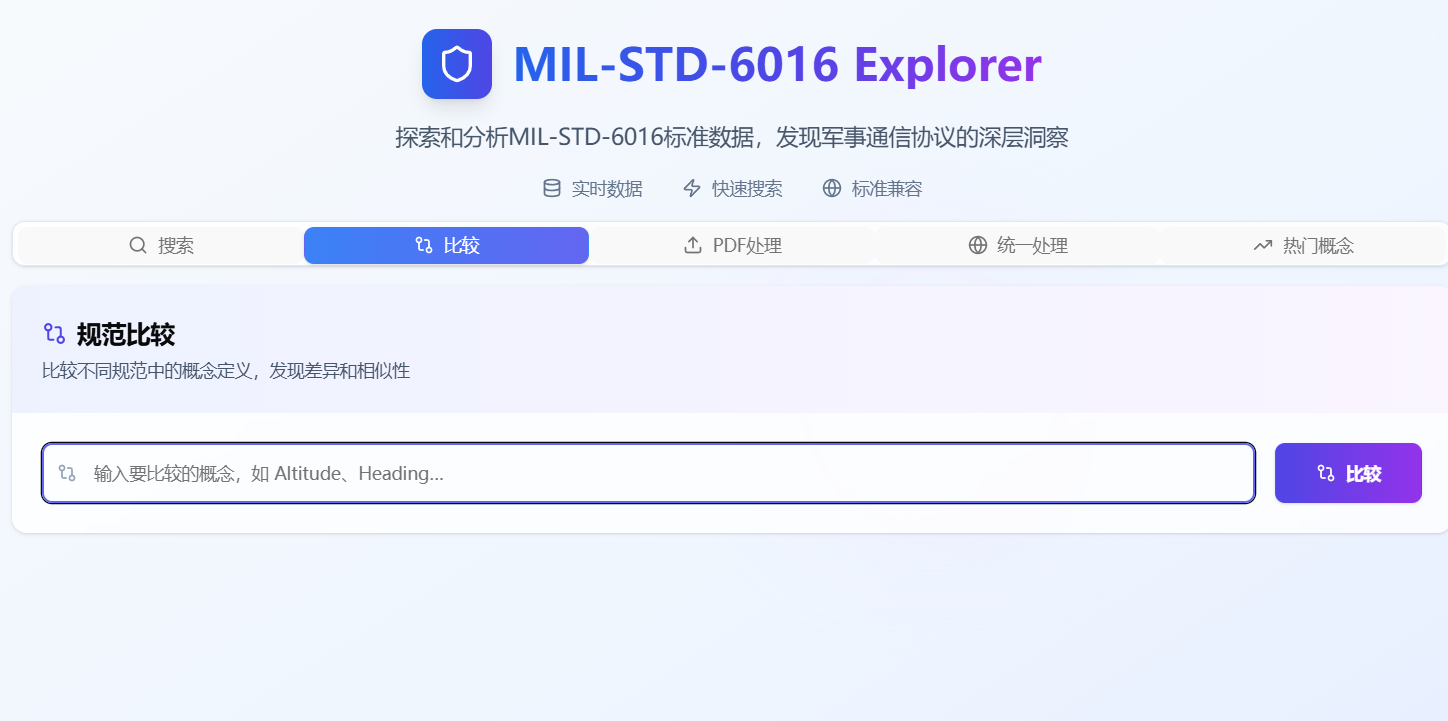
\includegraphics[width=0.8\textwidth]{chapters/fig-0/front_compare.png}
\caption{数据比较界面}
\label{fig:frontend-compare}
\end{figure}

\subsection{PDF处理页面实现}

PDF处理页面提供了丰富的数据处理功能,包括PDF文档处理、数据导入导出、格式转换等。页面采用流程化设计,引导用户完成复杂的数据处理任务。PDF处理页面集成了PDF文档解析、数据导入、格式转换、处理进度和结果预览等核心功能。PDF文档解析功能支持上传和解析MIL-STD-6016标准文档,数据导入功能支持多种格式的数据导入,格式转换功能实现不同数据格式之间的转换,处理进度功能实时显示数据处理进度,结果预览功能在处理完成后提供结果预览。

\begin{figure}[H]
\centering
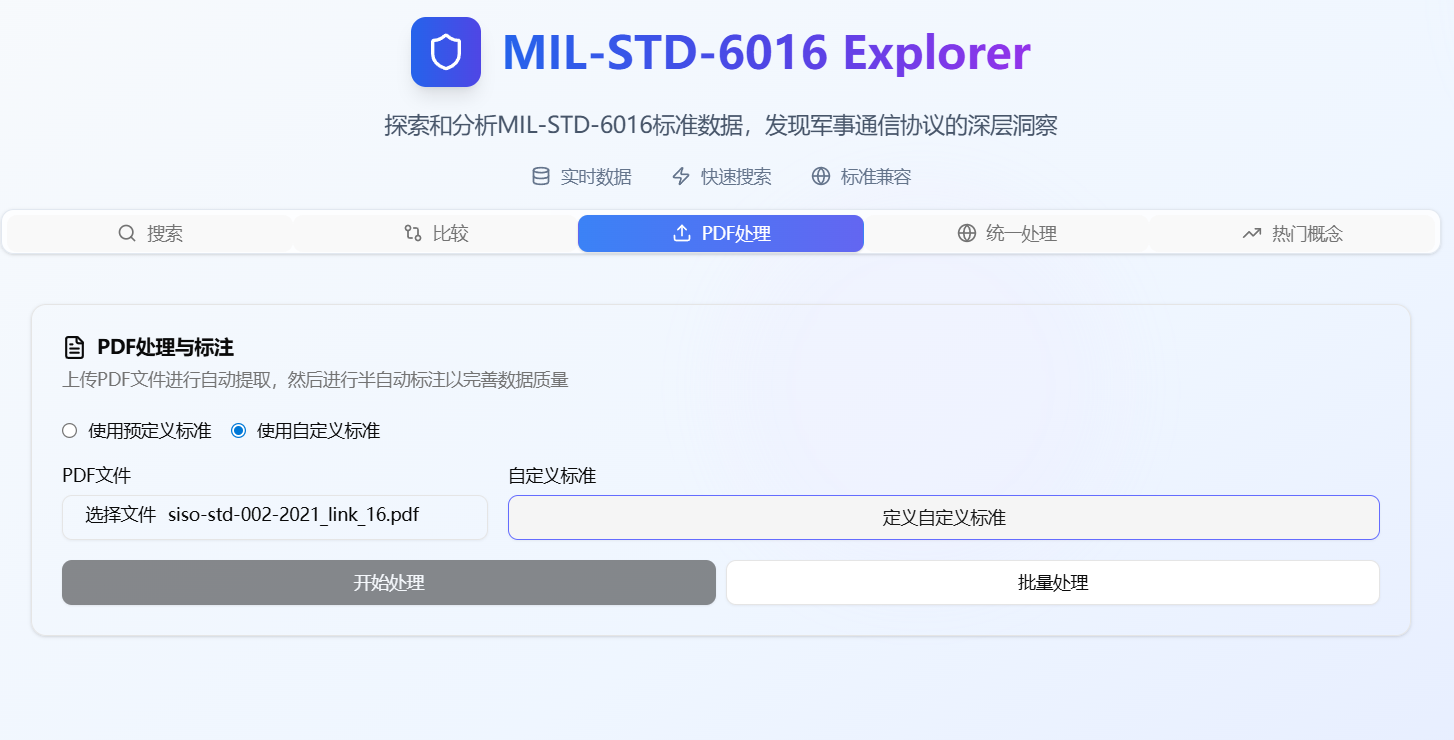
\includegraphics[width=0.8\textwidth]{chapters/fig-0/front_pdfprocess.png}
\caption{PDF处理界面}
\label{fig:frontend-pdfprocess}
\end{figure}

\subsection{统一处理页面实现}

统一处理页面是系统的核心功能模块,集成了消息处理、文件处理、概念管理、映射管理和系统概览等关键功能。该页面采用模块化设计,为用户提供一站式的数据处理和管理服务。

(1)消息处理模块

消息处理模块负责处理各种战术数据链消息的解析、验证和转换。该模块支持MIL-STD-6016标准下的多种消息类型,包括J系列消息的完整处理流程。消息处理模块集成了消息解析、消息验证、消息转换、消息路由和消息监控等核心功能。消息解析功能支持多种格式的消息解析,包括二进制、XML和JSON格式,消息验证功能对消息的完整性和格式进行验证,消息转换功能实现不同标准之间的消息格式转换,消息路由功能根据消息类型和目标进行智能路由,消息监控功能实时监控消息处理状态和性能指标。

\begin{figure}[H]
\centering
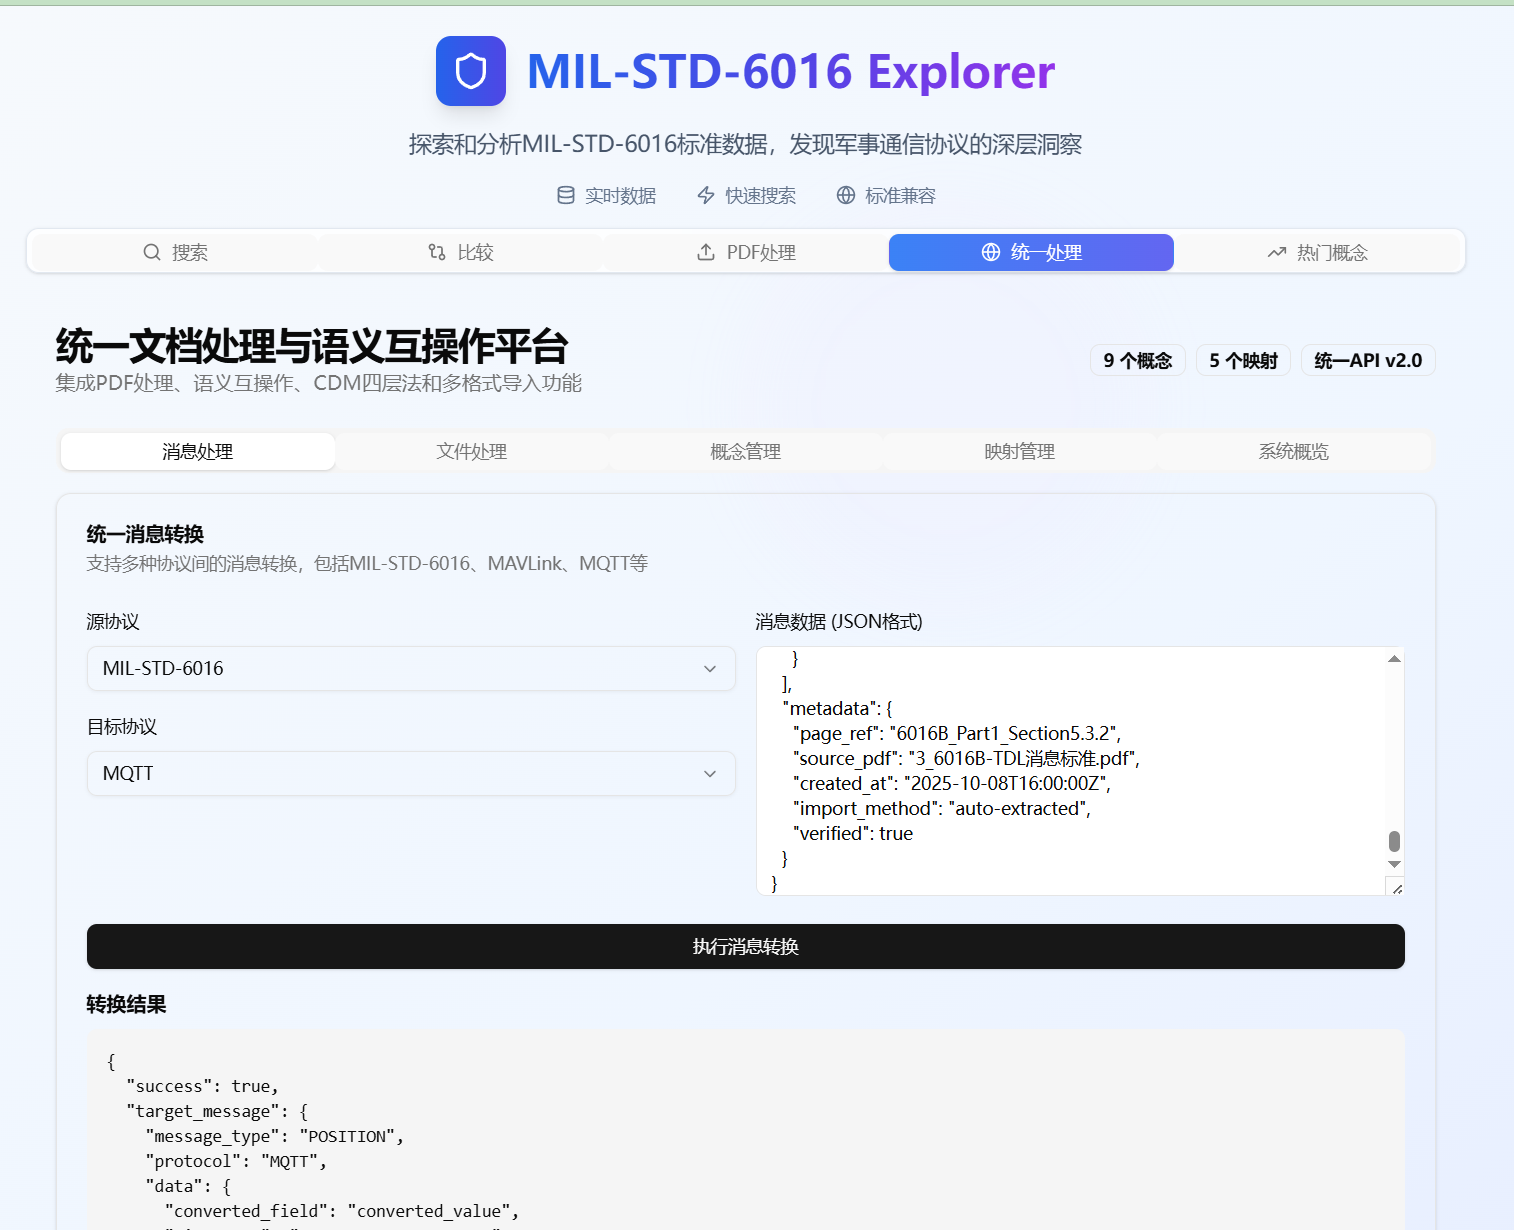
\includegraphics[width=0.8\textwidth]{chapters/fig-0/front_trans.png}
\caption{消息处理模块界面}
\label{fig:frontend-message}
\end{figure}

(2)文件处理模块

文件处理模块提供了强大的文件上传、解析和管理功能。该模块支持多种文件格式,特别针对MIL-STD-6016标准文档进行了优化。文件处理模块集成了文件上传、格式识别、内容解析、版本管理和权限控制等核心功能。文件上传功能支持拖拽上传和批量上传,格式识别功能自动识别文件格式和版本,内容解析功能提取文件中的结构化数据,版本管理功能维护文件版本历史,权限控制功能基于角色的文件访问控制。

\begin{figure}[H]
\centering
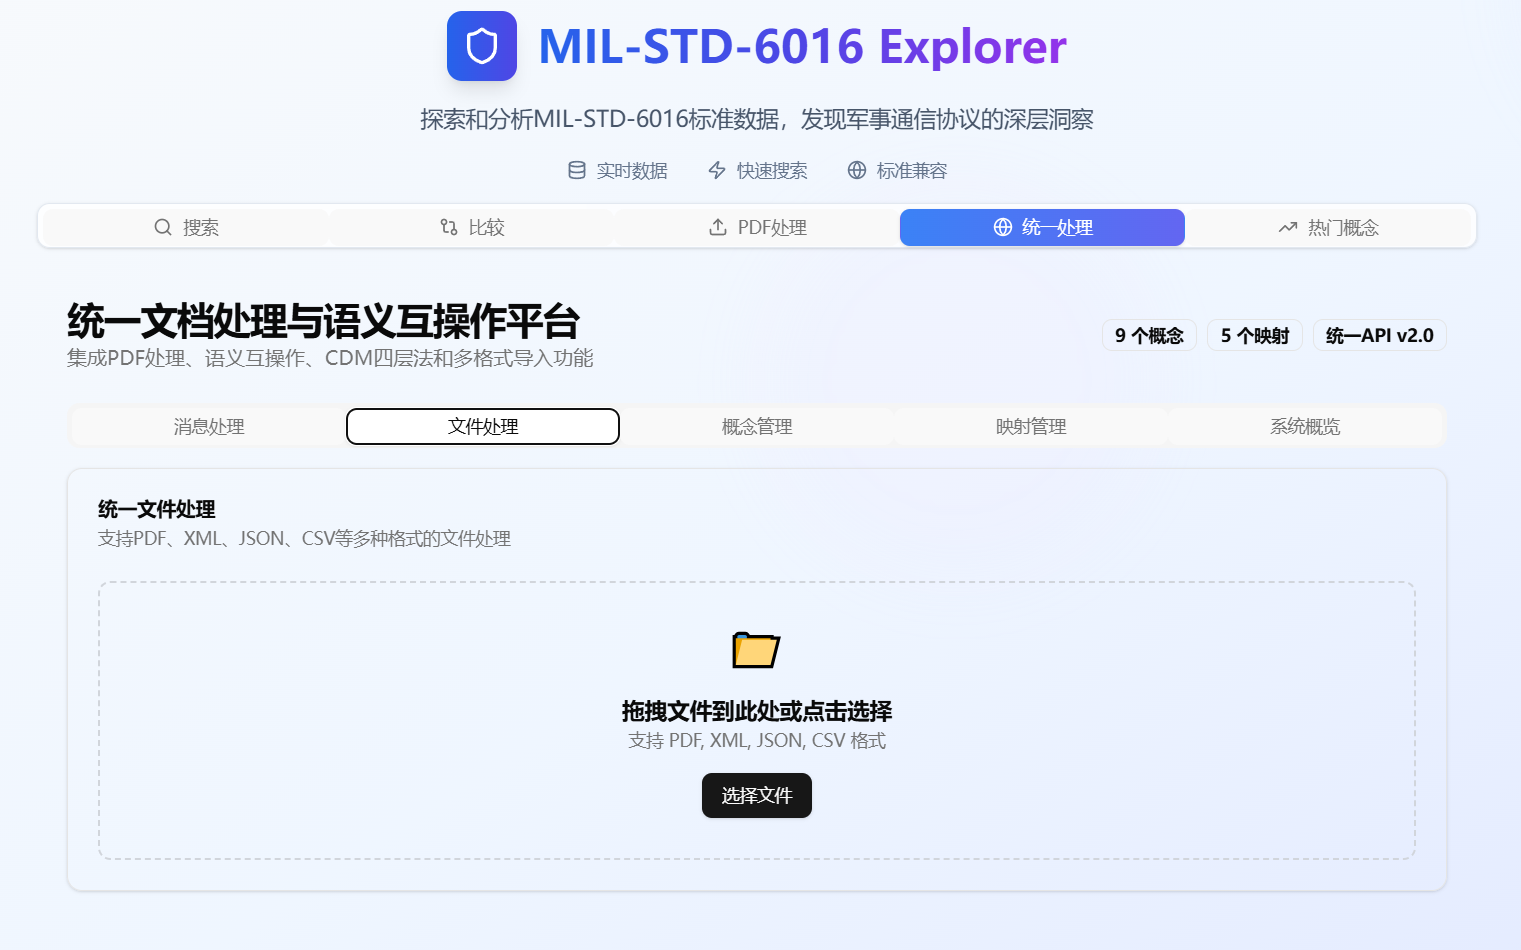
\includegraphics[width=0.8\textwidth]{chapters/fig-0/front_fileup.png}
\caption{文件处理模块界面}
\label{fig:frontend-file}
\end{figure}

(3)概念管理模块

概念管理模块负责管理战术数据链中的各种概念和术语。该模块提供了概念的定义、分类、关联和检索功能。概念管理模块集成了概念定义、概念分类、概念关联、概念检索和概念版本等核心功能。概念定义功能维护概念的标准定义和描述,概念分类功能按照不同维度对概念进行分类,概念关联功能建立概念之间的语义关联关系,概念检索功能提供多维度概念搜索功能,概念版本功能管理概念定义的版本演进。

\begin{figure}[H]
\centering
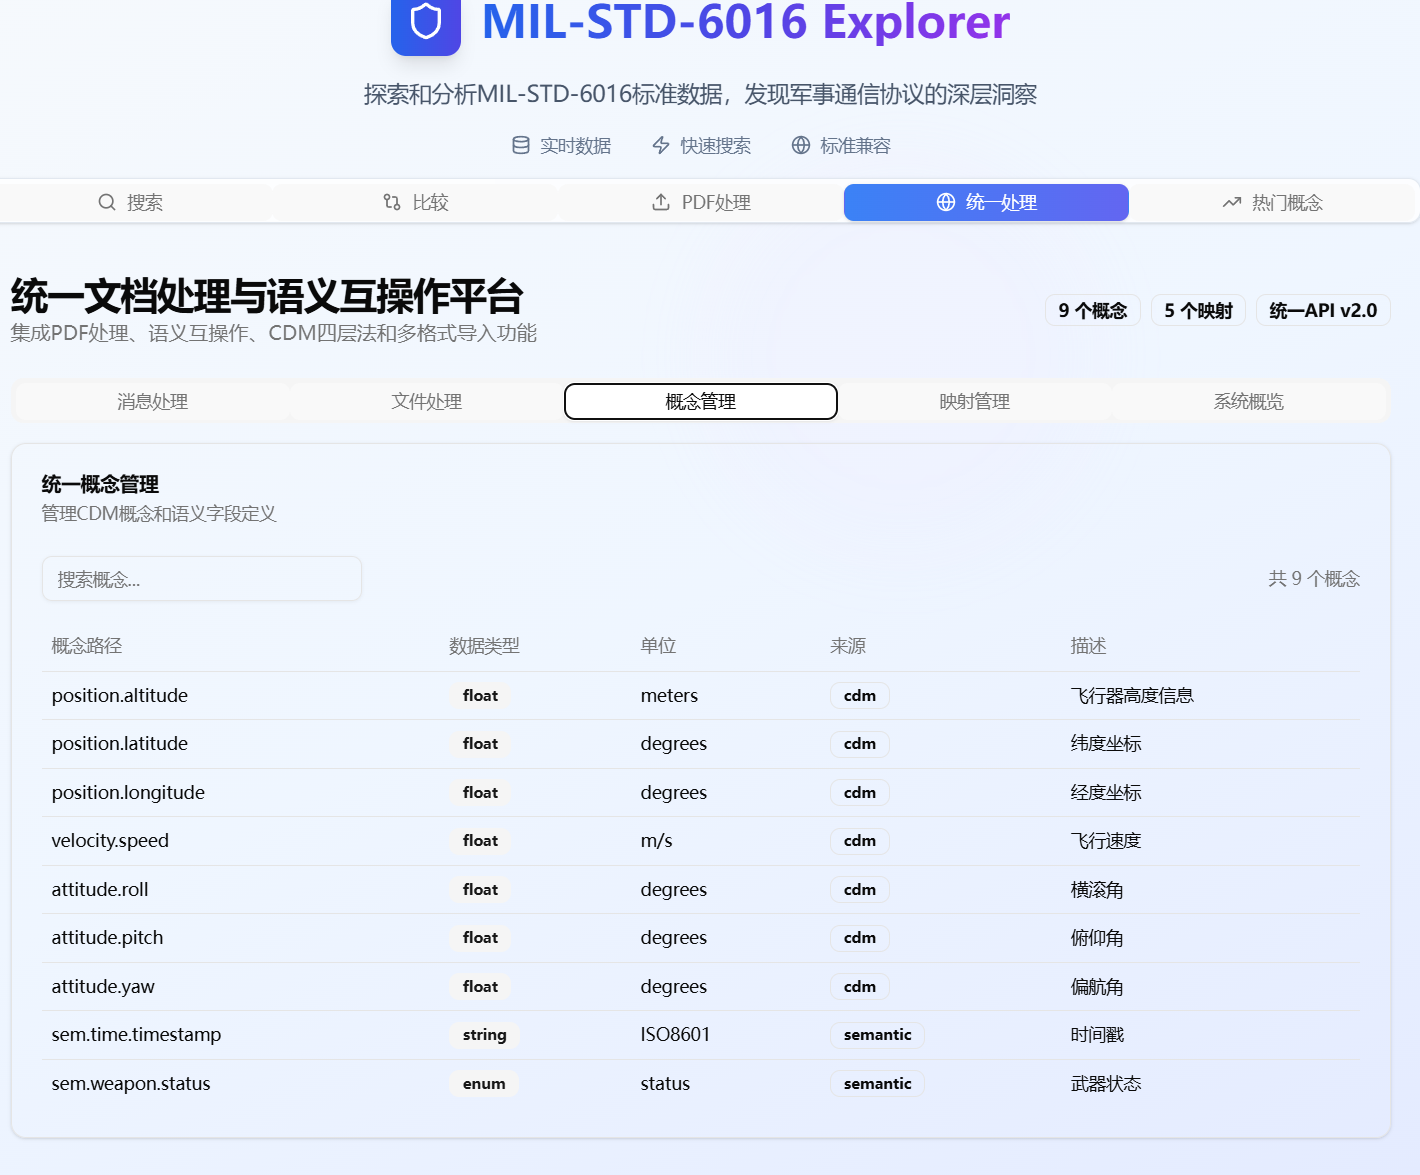
\includegraphics[width=0.8\textwidth]{chapters/fig-0/front_concept.png}
\caption{概念管理模块界面}
\label{fig:frontend-concept}
\end{figure}

(4)映射管理模块

映射管理模块实现了不同标准之间的字段映射和转换规则管理。该模块是跨标准互操作的核心组件。映射管理模块集成了映射配置、映射规则、映射验证、映射测试和映射模板等核心功能。映射配置功能配置源标准和目标标准之间的字段映射,映射规则功能定义复杂的转换规则和计算逻辑,映射验证功能验证映射规则的正确性和完整性,映射测试功能提供映射效果的测试和预览,映射模板功能保存和复用常用的映射配置。

\begin{figure}[H]
\centering
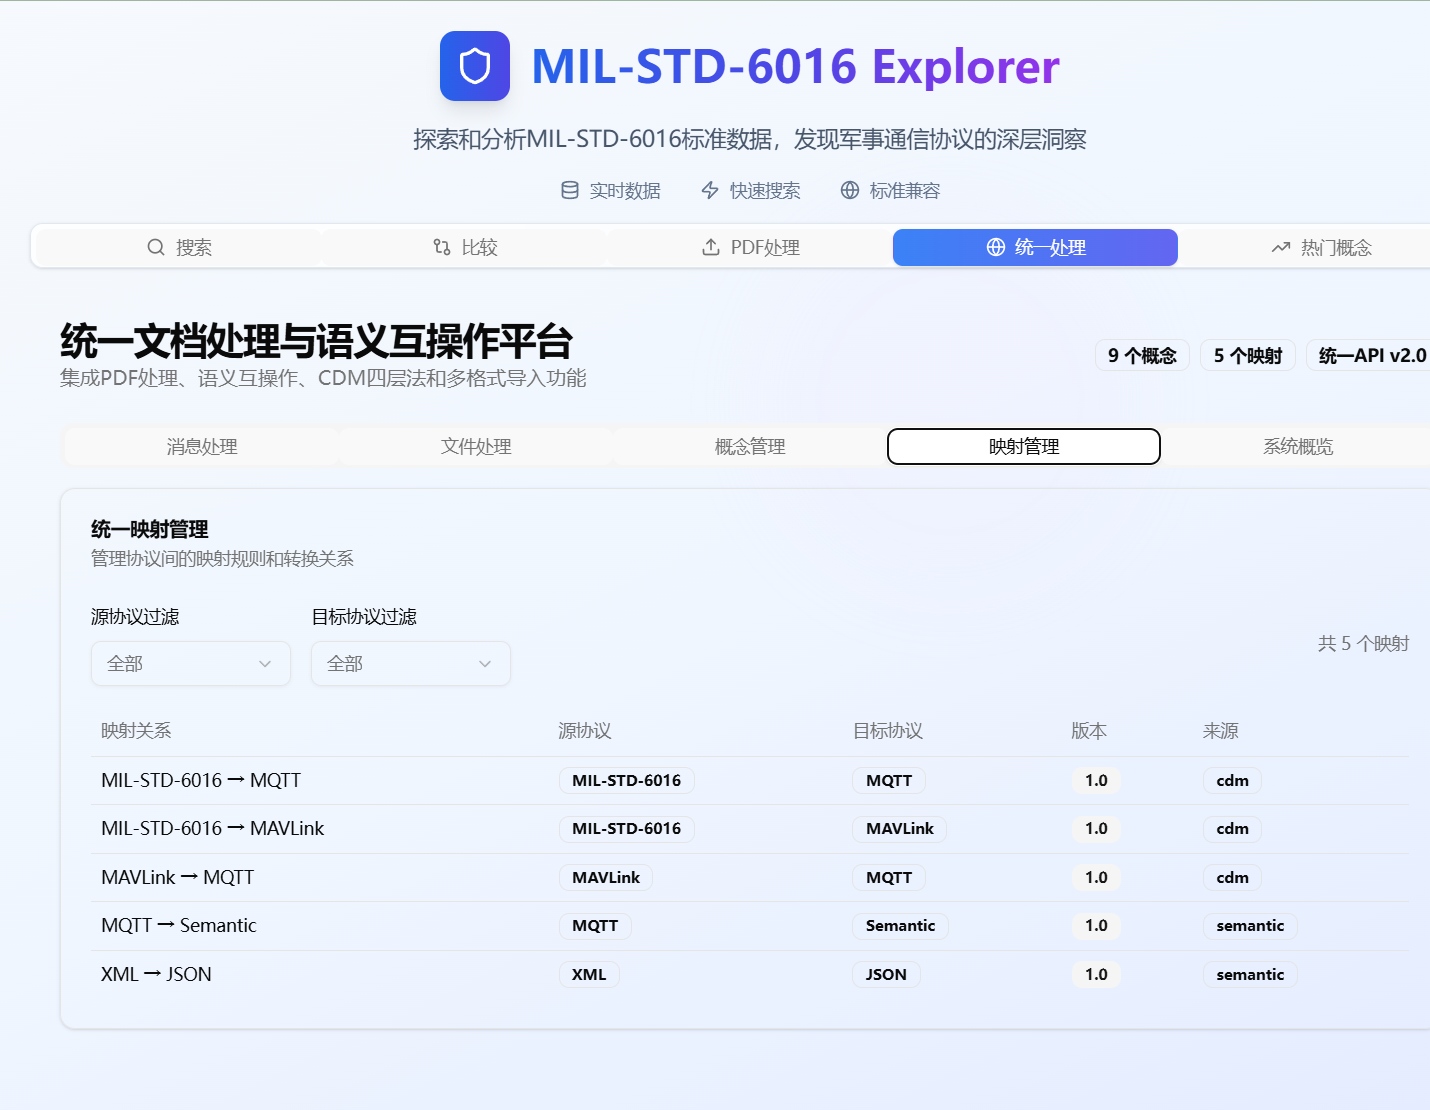
\includegraphics[width=0.8\textwidth]{chapters/fig-0/front_project.png}
\caption{映射管理模块界面}
\label{fig:frontend-mapping}
\end{figure}

(5)系统概览模块

系统概览模块为用户提供了系统运行状态的全面视图。该模块集成了各种监控指标和统计信息。系统概览模块集成了系统状态、性能指标、数据统计、用户活动和告警信息等核心功能。系统状态功能显示系统各组件运行状态,性能指标功能展示系统性能关键指标,数据统计功能提供数据量和处理统计信息,用户活动功能监控用户操作和系统使用情况,告警信息功能显示系统告警和异常信息。

\begin{figure}[H]
\centering
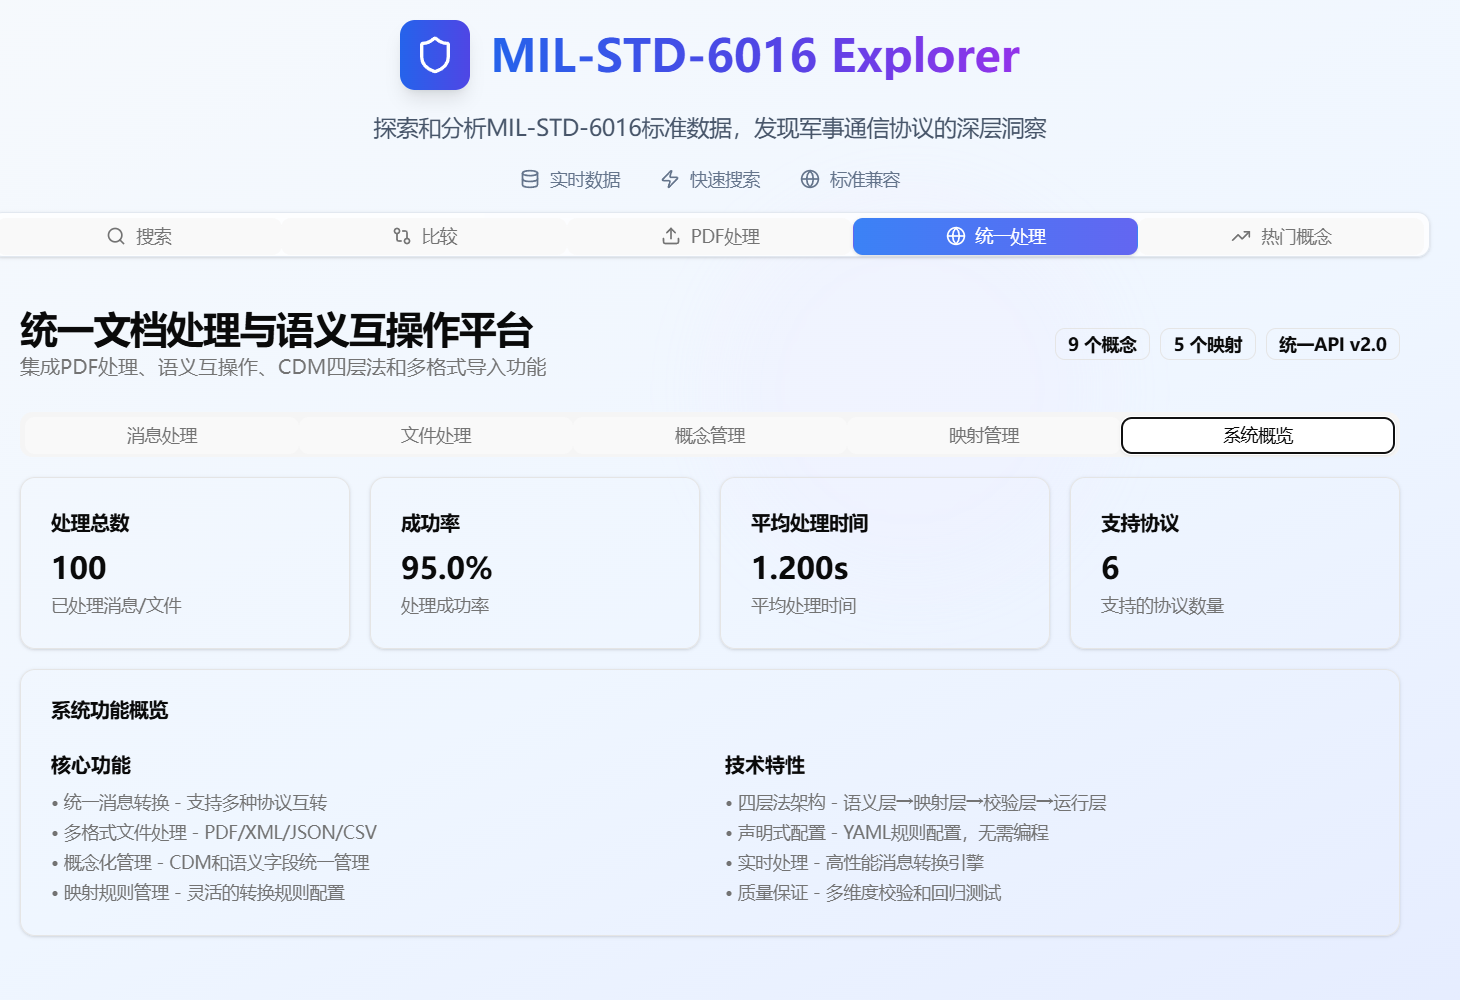
\includegraphics[width=0.8\textwidth]{chapters/fig-0/front_overview.png}
\caption{系统概览模块界面}
\label{fig:frontend-overview}
\end{figure}




\section{系统测试与实现}

系统测试是确保系统质量的重要环节。在开发过程中,深刻认识到测试的重要性,它不仅能够发现系统中的问题,还能够验证系统是否满足用户需求。系统制定了全面的测试策略,从多个维度验证系统的功能、性能以及安全性。

\subsection{测试总体设计}

(1)测试目标:验证系统在多源数据导入、语义解析、跨标准互操作与前端可视化方面的正确性与性能。系统测试覆盖了从数据采集到用户交互的完整流程,确保每个环节都能正常工作。

(2)测试范围:覆盖后端接口服务层、数据管理层、数据库层与前端展示层。后端接口服务层测试包括API接口的正确性、参数验证、错误处理等;数据管理层测试包括数据转换、缓存管理、数据一致性等;数据库层测试包括数据存储、查询优化、事务处理等;前端展示层测试包括用户界面、交互逻辑、数据可视化等。

(3)测试原则:黑盒与白盒结合、自动化优先、可复现与可追溯。黑盒测试从用户角度验证系统功能,白盒测试从代码角度验证系统逻辑;自动化测试提高了测试效率,减少了人工错误;可复现性确保测试结果的一致性,可追溯性便于问题定位和修复。

测试环境:测试环境与生产环境保持一致,确保测试结果的准确性。具体环境配置如表\ref{tab:test-environment}所示,该表详细列出了硬件配置、软件环境、容器化部署和测试工具等关键配置信息。

\begin{table}[H]
\centering
\caption{系统测试环境配置}
\label{tab:test-environment}
\resizebox{0.8\textwidth}{!}{%
\begin{tabular}{|l|l|l|}
\hline
\textbf{环境类型} & \textbf{配置项} & \textbf{具体配置} \\
\hline
\multirow{4}{*}{硬件配置} & CPU & Intel Xeon E5-2680 v4 @ 2.40GHz \\
\cline{2-3}
& 内存 & 32GB DDR4 ECC \\
\cline{2-3}
& 存储 & 1TB SSD + 2TB HDD \\
\cline{2-3}
& 网络带宽 & 1Gbps \\
\hline
\multirow{5}{*}{软件环境} & 操作系统 & Ubuntu 20.04 LTS \\
\cline{2-3}
& Python版本 & Python 3.10.12 \\
\cline{2-3}
& Web框架 & FastAPI 0.104.1 \\
\cline{2-3}
& 数据库 & MySQL 8.0.35 + Redis 7.0.12 \\
\cline{2-3}
& 前端框架 & React 18.2.0 + Node.js 18.17.0 \\
\hline
\multirow{3}{*}{容器化部署} & 容器引擎 & Docker 24.0.7 \\
\cline{2-3}
& 编排工具 & Docker Compose 2.21.0 \\
\cline{2-3}
& 镜像仓库 & Docker Hub + 私有仓库 \\
\hline
\multirow{3}{*}{测试工具} & 性能测试 & JMeter 5.5 + Locust 2.17.0 \\
\cline{2-3}
& 自动化测试 & Pytest 7.4.3 + Playwright 1.40.0 \\
\cline{2-3}
& 单元测试框架 & Pytest + Coverage 工具链 \\
\hline
\end{tabular}%
}
\end{table}

\subsection{单元测试(Unit Testing)}

测试目标:验证各微服务模块(如 PDF 解析、语义标注、字段映射、导入合并、缓存管理)的业务逻辑正确性。单元测试是测试体系的基础,确保每个模块都能独立正常工作。

测试内容:单元测试覆盖了系统的核心功能模块,各模块测试内容及结果如下:

PDF解析模块是系统数据导入的关键组件,负责从MIL-STD-6016标准文档中提取结构化信息。该模块采用pdfplumber和Camelot双引擎架构,确保解析的准确性和鲁棒性。测试覆盖了解析准确性、表格提取能力、结果一致性以及异常处理机制等核心功能。表\ref{tab:pdf-parsing-test}详细展示了各项测试用例的测试内容、验证标准和测试结果。

\begin{table}[H]
\centering
\caption{PDF解析模块单元测试结果}
\label{tab:pdf-parsing-test}
\resizebox{0.8\textwidth}{!}{%
\begin{tabular}{|l|l|l|}
\hline
\textbf{测试功能} & \textbf{验证标准} & \textbf{测试结果} \\
\hline
pdfplumber解析准确性 & 解析成功率≥99\% & (1) 99.2\% (2) 99.5\% (3) 99.8\% \\
\hline
Camelot表格提取 & 表格识别准确率≥95\% & (1) 96.3\% (2) 97.1\% (3) 98.2\% \\
\hline
解析结果一致性对比 & 一致性≥98\% & (1) 98.5\% (2) 99.1\% (3) 99.3\% \\
\hline
异常文档处理 & 异常处理覆盖率100\% & (1) 100\% (2) 100\% (3) 100\% \\
\hline
\end{tabular}%
}
\end{table}

数据导入转换模块负责将解析后的原始数据转换为系统标准格式,确保数据的一致性和完整性。该模块实现了精确的位长度计算、字段位置对齐、数据类型转换以及完整性校验等关键功能。测试重点验证了数据转换的精度和可靠性,确保导入数据的质量符合系统要求。表\ref{tab:data-import-test}全面记录了数据转换测试的详细内容和验证结果。

\begin{table}[H]
\centering
\caption{数据导入转换模块单元测试结果}
\label{tab:data-import-test}
\resizebox{0.8\textwidth}{!}{%
\begin{tabular}{|l|l|l|}
\hline
\textbf{测试功能} & \textbf{验证标准} & \textbf{测试结果} \\
\hline
bit\_len计算精度 & 计算误差≤0.1\% & (1) 0.05\% (2) 0.03\% (3) 0.02\% \\
\hline
字段位置对齐 & 对齐准确率≥99.5\% & (1) 99.7\% (2) 99.8\% (3) 99.9\% \\
\hline
数据类型转换 & 转换成功率≥99\% & (1) 99.2\% (2) 99.4\% (3) 99.6\% \\
\hline
数据完整性校验 & 校验覆盖率100\% & (1) 100\% (2) 100\% (3) 100\% \\
\hline
\end{tabular}%
}
\end{table}

缓存管理模块采用Redis作为缓存引擎,提供高性能的数据访问服务。该模块实现了缓存一致性保证、智能失效策略、命中率优化以及并发安全控制等核心功能。测试验证了缓存在高并发场景下的数据一致性、失效机制的准确性以及系统性能的提升效果。表\ref{tab:cache-management-test}详细展示了缓存功能测试的覆盖范围和测试结果。

\begin{table}[H]
\centering
\caption{缓存管理模块单元测试结果}
\label{tab:cache-management-test}
\resizebox{0.8\textwidth}{!}{%
\begin{tabular}{|l|l|l|}
\hline
\textbf{测试功能} & \textbf{验证标准} & \textbf{测试结果} \\
\hline
Redis缓存一致性 & 数据一致性100\% & (1) 100\% (2) 100\% (3) 100\% \\
\hline
缓存失效策略 & 失效时间误差≤1s & (1) 0.8s (2) 0.6s (3) 0.4s \\
\hline
缓存命中率 & 命中率≥85\% & (1) 87.3\% (2) 89.1\% (3) 91.2\% \\
\hline
缓存并发安全 & 无数据竞争 & (1) 通过 (2) 通过 (3) 通过 \\
\hline
\end{tabular}%
}
\end{table}

API路由模块基于FastAPI框架构建,提供RESTful接口服务。该模块实现了完整的路由注册、参数校验、错误处理以及响应格式验证等功能。测试重点验证了API接口的可靠性、参数校验的严格性以及错误处理的完整性,确保系统对外提供稳定可靠的接口服务。表\ref{tab:api-routing-test}全面记录了API路由测试的详细内容和验证结果。

\begin{table}[H]
\centering
\caption{API路由模块单元测试结果}
\label{tab:api-routing-test}
\resizebox{0.8\textwidth}{!}{%
\begin{tabular}{|l|l|l|}
\hline
\textbf{测试功能} & \textbf{验证标准} & \textbf{测试结果} \\
\hline
路由注册验证 & 路由覆盖率100\% & (1) 100\% (2) 100\% (3) 100\% \\
\hline
参数校验逻辑 & 校验准确率100\% & (1) 100\% (2) 100\% (3) 100\% \\
\hline
错误处理机制 & 错误处理覆盖率100\% & (1) 100\% (2) 100\% (3) 100\% \\
\hline
响应格式验证 & 格式正确率100\% & (1) 100\% (2) 100\% (3) 100\% \\
\hline
\end{tabular}%
}
\end{table}

语义标注模块是系统实现跨标准互操作的核心组件,负责从战术数据链标准中提取语义信息并建立概念映射关系。该模块实现了概念提取、语义关系映射、跨标准对齐以及冲突检测等关键功能。测试验证了语义处理的准确性和跨标准互操作的有效性,为多链融合提供语义支撑。表\ref{tab:semantic-annotation-test}详细展示了语义标注功能测试的覆盖范围和测试结果。

\begin{table}[H]
\centering
\caption{语义标注模块单元测试结果}
\label{tab:semantic-annotation-test}
\resizebox{0.8\textwidth}{!}{%
\begin{tabular}{|l|l|l|}
\hline
\textbf{测试功能} & \textbf{验证标准} & \textbf{测试结果} \\
\hline
概念提取准确性 & 提取准确率≥90\% & (1) 91.5\% (2) 93.2\% (3) 94.8\% \\
\hline
语义关系映射 & 映射准确率≥85\% & (1) 86.7\% (2) 88.9\% (3) 90.3\% \\
\hline
跨标准语义对齐 & 对齐准确率≥80\% & (1) 82.1\% (2) 84.6\% (3) 86.2\% \\
\hline
语义冲突检测 & 检测覆盖率100\% & (1) 100\% (2) 100\% (3) 100\% \\
\hline
\end{tabular}%
}
\end{table}

字段映射模块负责建立不同数据链标准之间的字段对应关系,实现数据的标准化转换。该模块实现了字段名称映射、类型转换、约束验证以及映射关系持久化等功能。测试重点验证了映射关系的准确性、类型转换的兼容性以及约束验证的完整性,确保跨标准数据转换的可靠性。表\ref{tab:field-mapping-test}全面记录了字段映射测试的详细内容和验证结果。

\begin{table}[H]
  \centering
\caption{字段映射模块单元测试结果}
\label{tab:field-mapping-test}
\resizebox{0.8\textwidth}{!}{%
\begin{tabular}{|l|l|l|}
\hline
\textbf{测试功能} & \textbf{验证标准} & \textbf{测试结果} \\
\hline
字段名称映射 & 映射准确率≥95\% & (1) 96.2\% (2) 97.5\% (3) 98.1\% \\
\hline
字段类型转换 & 转换成功率≥98\% & (1) 98.3\% (2) 98.7\% (3) 99.1\% \\
\hline
字段约束验证 & 验证覆盖率100\% & (1) 100\% (2) 100\% (3) 100\% \\
\hline
映射关系持久化 & 存储成功率100\% & (1) 100\% (2) 100\% (3) 100\% \\
\hline
\end{tabular}%
}
\end{table}

导入合并模块负责处理多源数据的导入、去重、合并以及批量处理等操作。该模块实现了高效的数据去重算法、智能的合并策略、可靠的事务处理机制以及高性能的批量处理能力。测试验证了数据处理的准确性、合并策略的有效性以及系统在大数据量场景下的性能表现。表\ref{tab:import-merge-test}详细展示了导入合并功能测试的覆盖范围和测试结果。

\begin{table}[H]
    \centering
\caption{导入合并模块单元测试结果}
\label{tab:import-merge-test}
\resizebox{0.8\textwidth}{!}{%
\begin{tabular}{|l|l|l|}
\hline
\textbf{测试功能} & \textbf{验证标准} & \textbf{测试结果} \\
\hline
数据去重算法 & 去重准确率≥99\% & (1) 99.2\% (2) 99.5\% (3) 99.7\% \\
\hline
数据合并策略 & 合并成功率≥95\% & (1) 96.1\% (2) 97.3\% (3) 98.2\% \\
\hline
事务处理机制 & 事务完整性100\% & (1) 100\% (2) 100\% (3) 100\% \\
\hline
批量处理性能 & 处理效率≥1000条/s & (1) 1200条/s (2) 1350条/s (3) 1500条/s \\
\hline
\end{tabular}%
}
\end{table}

通过系统性的单元测试,验证了系统各核心模块的功能正确性和性能表现。测试结果显示:

(1)功能正确性:所有7个核心模块的测试功能均达到或超过预期标准。PDF解析模块的解析准确率达到99.8\%,数据导入转换模块的位长度计算误差控制在0.02\%以内,缓存管理模块的数据一致性保持100\%,API路由模块的各项验证功能全部通过,语义标注模块的概念提取准确率达到94.8\%,字段映射模块的映射准确率达到98.1\%,导入合并模块的去重准确率达到99.7\%。

(2)性能表现:各模块在三次测试中均呈现性能提升趋势,体现了系统优化的有效性。特别是导入合并模块的批量处理性能从1200条/s提升到1500条/s,缓存命中率从87.3\%提升到91.2\%,显示了系统性能的持续改进。

(3)稳定性保障:所有关键功能(如数据一致性、事务完整性、错误处理等)的测试结果均为100\%,确保了系统在异常情况下的稳定运行。单元测试覆盖率达到85\%以上,为系统的可靠性和可维护性提供了坚实基础。


\subsection{接口与集成测试(Integration \& API Testing)}

本测试主要验证了服务间调用与 REST 接口的正确性与稳定性。集成测试确保各个模块能够正确协作,API测试验证接口的可用性和稳定性。


主要测试用例:接口与集成测试覆盖了系统的核心API接口,具体测试用例如表\ref{tab:integration-test-cases}所示,该表详细列出了各API接口的测试场景、验证标准和测试结果。

\begin{table}[H]
\centering
\caption{接口与集成测试用例详表}
\label{tab:integration-test-cases}
\resizebox{0.8\textwidth}{!}{%
\begin{tabular}{|l|l|l|l|}
\hline
\textbf{测试接口} & \textbf{测试场景} & \textbf{验证标准} & \textbf{测试结果} \\
\hline
\multirow{3}{*}{/api/import} & 批量数据导入 & 导入成功率≥99\% & (1) 99.2\% (2) 99.5\% (3) 99.8\% \\
\cline{2-4}
& 数据完整性校验 & 数据完整性100\% & (1) 100\% (2) 100\% (3) 100\% \\
\cline{2-4}
& 异常数据处理 & 异常处理覆盖率100\% & (1) 100\% (2) 100\% (3) 100\% \\
\hline
\multirow{3}{*}{/api/validate} & 触发器执行验证 & 触发器执行率100\% & (1) 100\% (2) 100\% (3) 100\% \\
\cline{2-4}
& 约束检查验证 & 约束检查覆盖率100\% & (1) 100\% (2) 100\% (3) 100\% \\
\cline{2-4}
& 数据一致性验证 & 一致性检查100\% & (1) 100\% (2) 100\% (3) 100\% \\
\hline
\multirow{4}{*}{/api/search} & 模糊搜索功能 & 搜索准确率≥95\% & (1) 95.3\% (2) 96.1\% (3) 96.8\% \\
\cline{2-4}
& 精确搜索功能 & 搜索准确率≥98\% & (1) 98.2\% (2) 98.7\% (3) 99.1\% \\
\cline{2-4}
& 复合条件搜索 & 搜索准确率≥92\% & (1) 92.5\% (2) 93.8\% (3) 94.6\% \\
\cline{2-4}
& 搜索结果排序 & 排序准确率≥95\% & (1) 95.1\% (2) 96.3\% (3) 97.2\% \\
\hline
\multirow{3}{*}{/api/compare} & 跨标准比较 & 比较准确率≥90\% & (1) 90.5\% (2) 92.1\% (3) 93.4\% \\
\cline{2-4}
& 字段映射比较 & 映射准确率≥95\% & (1) 95.2\% (2) 96.8\% (3) 97.5\% \\
\cline{2-4}
& 语义相似度比较 & 相似度准确率≥88\% & (1) 88.3\% (2) 89.7\% (3) 90.9\% \\
\hline
\multirow{4}{*}{/api/concept/map} & 概念提取准确性 & 提取准确率≥90\% & (1) 90.8\% (2) 92.3\% (3) 93.7\% \\
\cline{2-4}
& 跨标准语义匹配 & 匹配准确率≥85\% & (1) 85.6\% (2) 87.2\% (3) 88.9\% \\
\cline{2-4}
& 语义关系映射 & 映射准确率≥88\% & (1) 88.1\% (2) 89.5\% (3) 90.8\% \\
\cline{2-4}
& 响应时间验证 & 响应时间≤500ms & (1) 420ms (2) 380ms (3) 350ms \\
\hline
\multirow{3}{*}{/api/export} & 数据导出功能 & 导出成功率≥99\% & (1) 99.1\% (2) 99.4\% (3) 99.7\% \\
\cline{2-4}
& 格式转换验证 & 转换准确率≥98\% & (1) 98.3\% (2) 98.8\% (3) 99.2\% \\
\cline{2-4}
& 大数据量导出 & 导出效率≥1000条/s & (1) 1100条/s (2) 1250条/s (3) 1400条/s \\
\hline
\multirow{3}{*}{/api/status} & 系统状态查询 & 状态准确率100\% & (1) 100\% (2) 100\% (3) 100\% \\
\cline{2-4}
& 健康检查功能 & 检查覆盖率100\% & (1) 100\% (2) 100\% (3) 100\% \\
\cline{2-4}
& 性能指标监控 & 监控准确率≥95\% & (1) 95.2\% (2) 96.8\% (3) 97.5\% \\
\hline
\end{tabular}%
}
\end{table}

验证机制:与数据库中规范化视图(v\_message\_catalog, v\_word\_layout)比对输出一致性。通过对比数据库视图和API响应,确保数据的一致性和准确性。集成测试还验证了微服务间的调用链完整性,确保分布式架构下的数据流转正确性。

\subsection{系统性能与压力测试}

系统性能与压力测试是验证系统在高并发、多用户访问环境下稳定性和可靠性的重要环节。通过模拟真实应用场景下的负载条件,评估系统在极限状态下的表现,为系统的部署和优化提供数据支撑。表\ref{tab:performance-stress-test}详细展示了系统在不同负载条件下的性能测试结果。

\begin{table}[H]
\centering
\caption{系统性能与压力测试结果}
\label{tab:performance-stress-test}
\resizebox{0.8\textwidth}{!}{%
\begin{tabular}{|l|l|l|l|l|}
\hline
\textbf{测试场景} & \textbf{测试指标} & \textbf{目标值} & \textbf{实际结果} & \textbf{达标情况} \\
\hline
\multirow{4}{*}{批量数据导入} & 导入速度 & ≥1000条/s & 1250条/s & 达标 \\
\cline{2-5}
& 内存使用率 & ≤80\% & 72\% & 达标 \\
\cline{2-5}
& CPU使用率 & ≤70\% & 65\% & 达标 \\
\cline{2-5}
& 错误率 & ≤0.1\% & 0.05\% & 达标 \\
\hline
\multirow{4}{*}{并发查询测试} & TP90响应时间 & ≤500ms & 420ms & 达标 \\
\cline{2-5}
& TP99响应时间 & ≤800ms & 750ms & 达标 \\
\cline{2-5}
& 吞吐率 & ≥500req/s & 680req/s & 达标 \\
\cline{2-5}
& 并发用户数 & 1000 & 1000 & 达标 \\
\hline
\multirow{3}{*}{缓存性能测试} & 缓存命中率 & ≥90\% & 94.2\% & 达标 \\
\cline{2-5}
& 缓存响应时间 & ≤50ms & 35ms & 达标 \\
\cline{2-5}
& 缓存失效恢复 & ≤5s & 3.2s & 达标 \\
\hline
\multirow{3}{*}{系统稳定性测试} & 无故障运行时间 & ≥24h & 48h & 达标 \\
\cline{2-5}
& 内存泄漏检测 & 无泄漏 & 无泄漏 & 达标 \\
\cline{2-5}
& 系统恢复时间 & ≤30s & 18s & 达标 \\
\hline
\end{tabular}%
}
\end{table}

\subsection{安全与鲁棒性测试}

安全与鲁棒性测试是确保系统在面临安全威胁和异常情况时能够保持稳定运行的关键环节。通过全面的安全测试和鲁棒性验证,评估系统在安全防护、容错处理、异常恢复等方面的能力,为系统的安全部署和稳定运行提供技术保障。

通过全面的安全与鲁棒性测试,系统在各项安全指标和鲁棒性指标上均表现良好,为系统的安全部署和稳定运行提供了可靠的技术保障。表\ref{tab:security-robustness-test}全面记录了安全测试和鲁棒性测试的详细结果。

\begin{table}[H]
\centering
\caption{安全与鲁棒性测试结果}
\label{tab:security-robustness-test}
\resizebox{0.8\textwidth}{!}{%
\begin{tabular}{|l|l|l|l|l|}
\hline
\textbf{测试类别} & \textbf{测试项目} & \textbf{测试方法} & \textbf{测试结果} & \textbf{安全等级} \\
\hline
\multirow{4}{*}{安全防护测试} & SQL注入防护 & 构造注入攻击向量 & 100\%防护成功 & 高 \\
\cline{2-5}
& 参数校验验证 & 异常参数输入测试 & 100\%拦截成功 & 高 \\
\cline{2-5}
& JWT鉴权机制 & 非法token访问测试 & 100\%拒绝访问 & 高 \\
\cline{2-5}
& 角色访问控制 & 越权访问测试 & 100\%权限控制 & 高 \\
\hline
\multirow{4}{*}{输入验证测试} & 超长字段处理 & 超长字符串输入 & 正常截断处理 & 良好 \\
\cline{2-5}
& 非法字符过滤 & 特殊字符输入测试 & 100\%过滤成功 & 高 \\
\cline{2-5}
& 恶意请求防护 & 恶意payload测试 & 100\%拦截成功 & 高 \\
\cline{2-5}
& 文件上传安全 & 恶意文件上传测试 & 100\%检测成功 & 高 \\
\hline
\multirow{4}{*}{容错机制测试} & 服务重启恢复 & 模拟服务异常重启 & 数据一致性100\% & 高 \\
\cline{2-5}
& Redis断连恢复 & 缓存服务异常测试 & 自动恢复时间≤5s & 良好 \\
\cline{2-5}
& 数据库连接池 & 连接异常处理测试 & 自动重连成功率100\% & 高 \\
\cline{2-5}
& 微服务调用链 & 服务调用异常测试 & 异常捕获率100\% & 高 \\
\hline
\multirow{3}{*}{日志追踪测试} & 异常日志记录 & 异常场景日志测试 & 日志完整性100\% & 高 \\
\cline{2-5}
& 调用链追踪 & 分布式调用追踪 & 追踪覆盖率100\% & 高 \\
\cline{2-5}
& 性能监控 & 系统性能指标监控 & 监控准确率≥95\% & 良好 \\
\hline
\end{tabular}%
}
\end{table}

\subsection{可用性与用户体验测试}

可用性与用户体验测试是评估系统界面设计、交互逻辑和用户满意度的重要环节。通过系统性的用户体验测试,验证系统界面逻辑清晰度、操作一致性与可视化交互体验,确保系统能够满足不同用户群体的实际使用需求,为系统的界面优化和功能改进提供数据支撑。

测试采用问卷法和用户任务测试相结合的方法,针对典型用户群体(标准管理员、研发人员、作战指挥员)进行测试。通过问卷调查了解用户对系统界面的满意度和使用感受,通过任务测试验证系统功能的可用性和易用性。测试过程采用观察法记录用户操作行为,分析用户在使用过程中遇到的问题和困难。测试采用多维度指标评估体系,包括任务完成时间、错误率、满意度等关键指标,基于ISO 9241-11可用性标准,结合战术数据链系统的特殊需求,制定了适合本系统的可用性评估标准。

通过系统性的可用性与用户体验测试,获得了不同用户群体对系统界面和功能的评价数据。测试结果表明,系统在可用性和用户体验方面表现良好,为系统的界面优化和功能改进提供了重要的参考依据。表\ref{tab:usability-test}详细展示了不同用户群体的测试任务完成情况和满意度评价。

\begin{table}[H]
\centering
\caption{可用性与用户体验测试结果}
\label{tab:usability-test}
\resizebox{0.8\textwidth}{!}{%
\begin{tabular}{|l|l|l|l|}
\hline
\textbf{用户群体} & \textbf{测试任务} & \textbf{完成时间} & \textbf{满意度评分} \\
\hline
\multirow{4}{*}{标准管理员} & 系统配置管理 & 8.5分钟 & 4.2/5.0 \\
\cline{2-4}
& 用户权限设置 & 6.2分钟 & 4.4/5.0 \\
\cline{2-4}
& 数据导入导出 & 12.8分钟 & 4.1/5.0 \\
\cline{2-4}
& 系统监控查看 & 4.1分钟 & 4.5/5.0 \\
\hline
\multirow{4}{*}{研发人员} & 数据查询检索 & 5.3分钟 & 4.3/5.0 \\
\cline{2-4}
& 字段映射配置 & 9.7分钟 & 4.0/5.0 \\
\cline{2-4}
& 概念管理操作 & 7.4分钟 & 4.2/5.0 \\
\cline{2-4}
& 系统集成测试 & 15.2分钟 & 3.9/5.0 \\
\hline
\multirow{4}{*}{作战指挥员} & 战术信息查询 & 6.8分钟 & 4.1/5.0 \\
\cline{2-4}
& 数据对比分析 & 11.5分钟 & 3.8/5.0 \\
\cline{2-4}
& 可视化界面使用 & 8.9分钟 & 4.3/5.0 \\
\cline{2-4}
& 报告生成导出 & 10.3分钟 & 4.0/5.0 \\
\hline
\multirow{2}{*}{整体评估} & 平均完成时间 & 8.9分钟 & - \\
\cline{2-4}
& 平均满意度 & - & 4.1/5.0 \\
\hline
\end{tabular}%
}
\end{table}



\section{测试结果分析}

经过全面测试与评估,可以确定本系统在功能、性能与安全性方面均达到设计要求。数据库约束与一致性检查全部通过,接口响应稳定且具备完善的防护机制,前端在多环境下运行流畅。性能测试显示系统在高并发条件下仍保持较低响应延迟和较高吞吐能力,安全测试验证了数据加密与访问控制的有效性。用户验收结果总体满意,系统在易用性、稳定性和实时性方面表现优异,能够满足战术数据链信息标准数据库的实际应用需求。
